\clearpage
\section[Fully-coupled model]{Solving a problem using a Fully-Coupled Model}\label{tutorial-coupled}

The process of solving a problem using \Dumux can be roughly divided into four parts:
\begin{enumerate}
 \item The geometry of the problem and correspondingly a grid have to be defined.
 \item Material properties and constitutive relationships have to be defined.
 \item Boundary conditions as well as initial conditions have to be defined.
 \item A suitable model has to be chosen.
\end{enumerate}

The problem that is solved in this tutorial is illustrated in figure \ref{tutorial-coupled:problemfigure}. A rectangular domain with no flow boundaries on the top and on the bottom, which is initially saturated with oil, is considered. Water infiltrates from the left side into the domain. Gravity effects as well as capillarity effects are neglected.

\begin{figure}[h]
\psfrag{x}{x}
\psfrag{y}{y}
\psfrag{no flow}{no flow}
\psfrag{water}{\textbf{water}}
\psfrag{oil}{\textcolor{white}{\textbf{oil}}}
\psfrag{p_w = 2 x 10^5 [Pa]}{$p_w = 2 \times 10^5$ [Pa]}
\psfrag{p_w_initial = 2 x 10^5 [Pa]}{\textcolor{white}{\textbf{$\mathbf{p_{w_{initial}} = 2 \times 10^5}$ [Pa]}}}
\psfrag{S_n = 0}{$S_n = 0$}
\psfrag{S_n_initial = 0}{\textcolor{white}{$\mathbf{S_{n_{initial}} = 1}$}}
\psfrag{q_w = 0 [kg/m^2s]}{$q_w = 0$ $\left[\frac{\textnormal{kg}}{\textnormal{m}^2 \textnormal{s}}\right]$}
\psfrag{q_n = -3 x 10^-4 [kg/m^2s]}{$q_n = -3 \times 10^-4$ $\left[\frac{\textnormal{kg}}{\textnormal{m}^2 \textnormal{s}}\right]$}
\centering
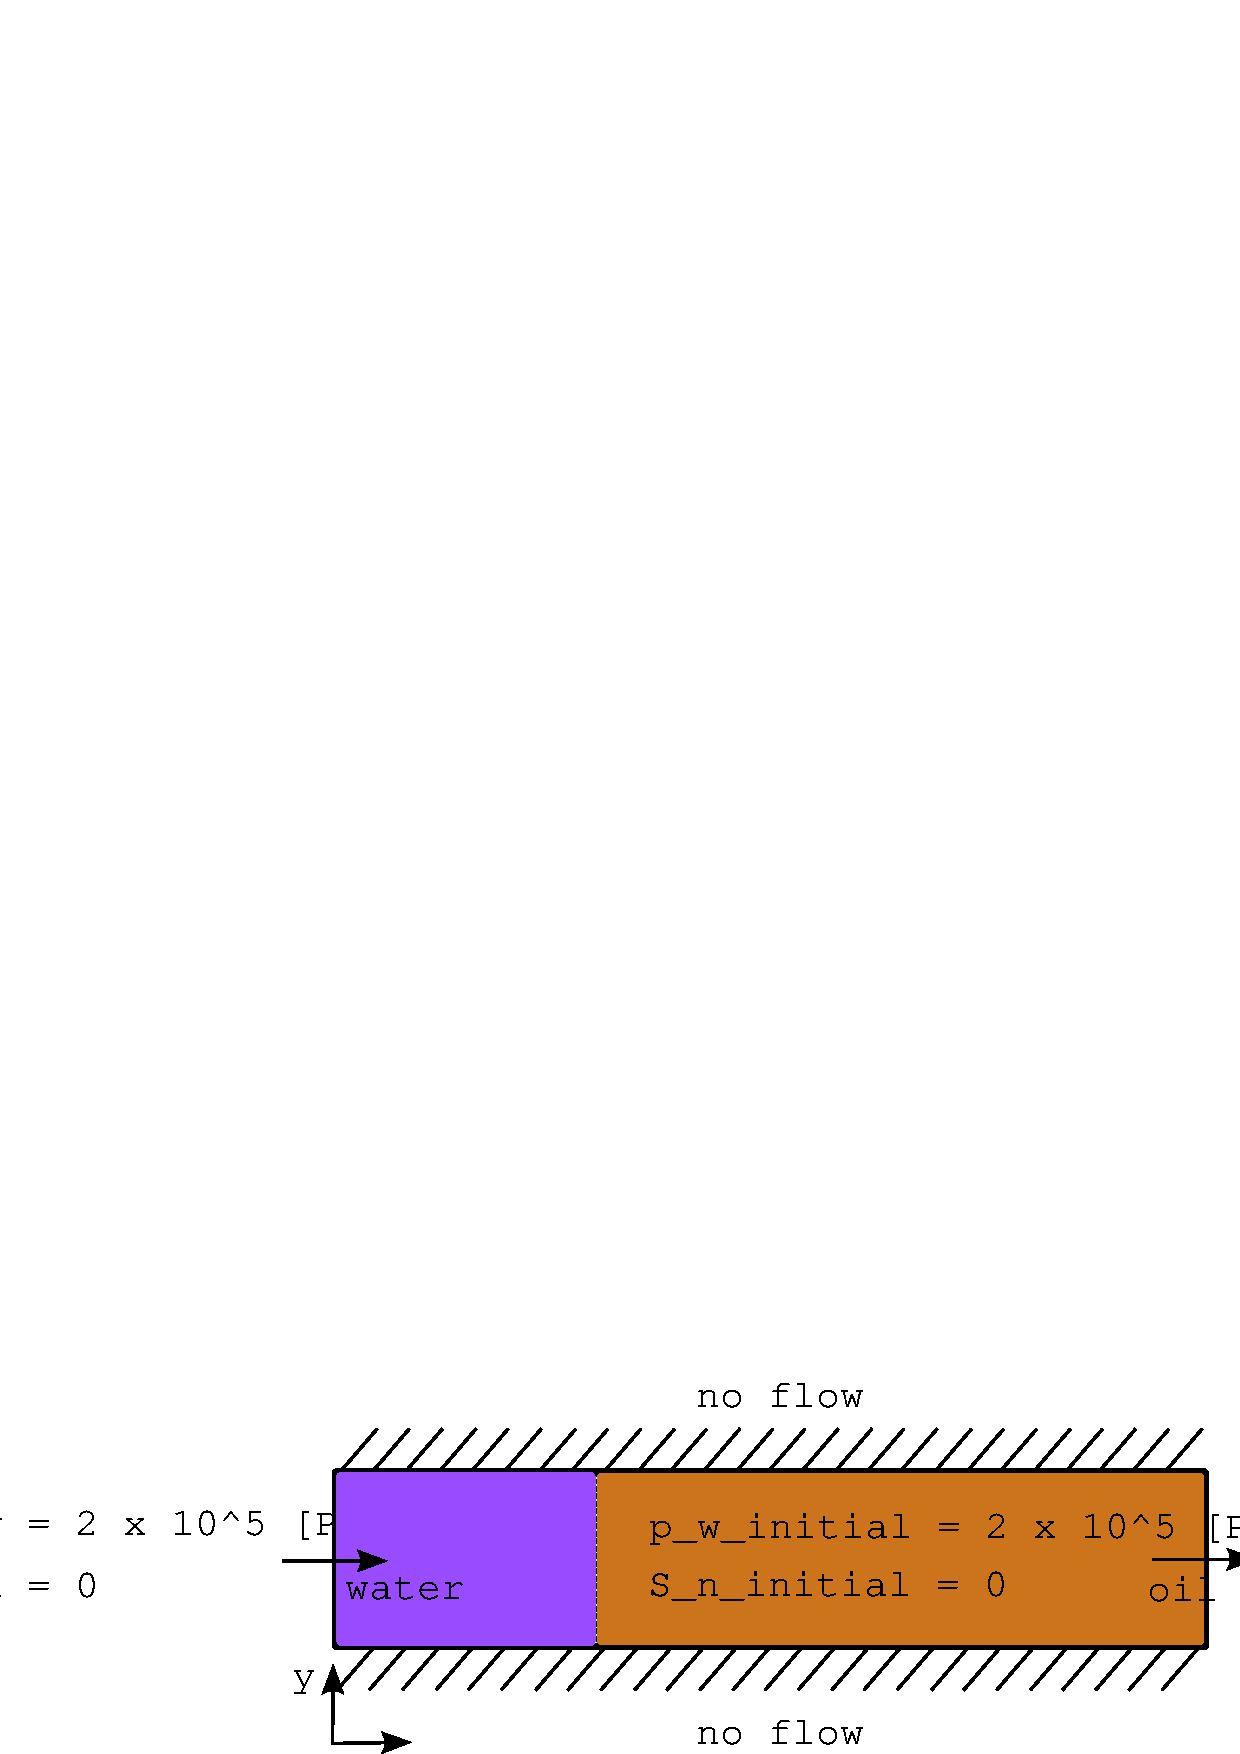
\includegraphics[width=0.9\linewidth,keepaspectratio]{EPS/tutorial-problemconfiguration}
\caption{Geometry of the tutorial problem with initial and boundary conditions.}\label{tutorial-coupled:problemfigure}
\end{figure}

The equations that are solved here are the mass balances of oil and
water:
\begin{align}
  \label{massbalancewater}
  \frac {\partial (\phi \, S_{w}\, \varrho_{w})}{\partial t}
  +
  \nabla \cdot \left( \varrho_{w} \, \frac{k_{rw}}{\mu_{w}} \, \mathbf{K}\;\nabla p \right)
  -
  q
  & =
  0 \\
  \label{massbalanceoil}
  \frac {\partial (\phi \, S_{o}\, \varrho_{o})}{\partial t}
  +
  \nabla \cdot \left( \varrho_{o} \, \frac{k_{ro}}{\mu_{o}} \, \mathbf{K}\;\nabla p \right)
  -
  q 
  & =
  0
\end{align}

\subsection{The main file}

Listing \ref{tutorial-coupled:mainfile} shows the main file
\texttt{tutorial/tutorial\_coupled.cc} for the coupled twophase
model. This file needs to be executed to solve the problem described
above.

\begin{lst}[File tutorial/tutorial\_coupled.cc]\label{tutorial-coupled:mainfile} \mbox{}
  \lstinputlisting[basicstyle=\ttfamily\scriptsize,numbers=left,
  numberstyle=\tiny, numbersep=5pt, firstline=18]{../../tutorial/tutorial_coupled.cc}
\end{lst}

From line \ref{tutorial-coupled:include-begin} to line
\ref{tutorial-coupled:include-end} the Dune and \Dumux files which
contain the needed functions and classes are included.

At line \ref{tutorial-coupled:set-type-tag} the type tag of the
problem which is going to be simulated is set. All other data types
can be retrieved by the \Dumux property system and only depend on this
single type tag. Retrieving them is done between line
\ref{tutorial-coupled:retrieve-types-begin} and
\ref{tutorial-coupled:retrieve-types-end}. For an introduction to the
property system, see section \textbf{TODO}.

The first thing which should be done at run time is to initialize the
message passing interface using DUNE's \texttt{MPIHelper} class. Line
\ref{tutorial-coupled:init-mpi} line is essential if the simulation is
intended to be run on more than one processor at the same time. Next,
the command line arguments are parsed starting at line
\ref{tutorial-coupled:parse-args-begin} until line
\ref{tutorial-coupled:parse-args-end}. In this case, we check if and
at which time a previous run of the simulation should be restarted, we
parse the initial size of a time step and the time when the simulation
ends.

After this, a grid is created on line
\ref{tutorial-coupled:create-grid} and the problem is instantiated for
its leaf grid view on line \ref{tutorial-coupled:instantiate-problem}.
Finally, on line \ref{tutorial-coupled:restart} a state written to
disk by a previous simulation run is restored on request by the user
and the simulation proceedure is started at line
\ref{tutorial-coupled:execute}.

\subsection{The problem class}

When solving a problem using \Dumux, the most important file is the
so-called \textit{problem file} as shown in listing
\ref{tutorial-coupled:problemfile} of
\texttt{tutorialproblem\_coupled.hh}.

\begin{lst}[File tutorial/tutorialproblem\_coupled.hh]\label{tutorial-coupled:problemfile} \mbox{}
\lstinputlisting[basicstyle=\ttfamily\scriptsize,numbers=left,
numberstyle=\tiny, numbersep=5pt, firstline=17]{../../tutorial/tutorialproblem_coupled.hh}
\end{lst}

First, a new type tag is created for the problem on line
\ref{tutorial-coupled:create-type-tag}.  In this case, the new type
tag inherits all properties defined for the \texttt{BoxTwoP} type tag,
which means that for this problem the two-phase box model is chosen as
discretization scheme. On line \ref{tutorial-coupled:set-problem}, a
problem class is attached to the new type tag, while the grid which
going to be used is defined on line \ref{tutorial-coupled:set-grid} --
in this case it's \texttt{SGrid}.  Since in Dune, there's no uniform
mechanism to allocate grids, the \texttt{Grid} property also contains
a static \texttt{create()} method which provides just that. Next,
fluids used as wetting phase and non-wetting phase as well as the soil
properties are specified on lines \ref{tutorial-coupled:set-wetting},
\ref{tutorial-coupled:set-nonwetting} and
\ref{tutorial-coupled:set-soil}. The final property on line line
\ref{tutorial-coupled:gravity} is optional and tells the model not to
use gravity.

Parameters which are specific to a set-up -- like boundary and initial
conditions, source terms or temperature within the domain -- but are
required to solve the differential equations of the models are
specified via a \textit{problem} class. If the two-phase box model is
used, this class must be derived from \texttt{TwoPBoxProblem} as done
on line \ref{tutorial-coupled:def-problem}.

The problem class always has at least five methods:
\begin{itemize}
\item A method \texttt{boundaryTypes()} specifying the kind of
  boundary conditions to be used for a boundary segment
\item A method \texttt{dirichlet()} specifying the actual values for
  the Dirichlet conditions on a boundary segment
\item A method \texttt{neumann()} specifying the actual values for
  the Neumann conditions on a boundary segment
\item A method for source or sink terms called \texttt{source}
\item A method called \texttt{initial()} for specifying the initial
  condition.
\end{itemize}

Methods which make statements about boundary segments of the grid (i.e. 
\texttt{boundaryTypes()}, \texttt{dirichlet()} and \texttt{neumann()}) get 
six parameters:
\begin{description}
\item[values:] A vector which stores the result of the method. What
  the values in this vector means is dependent on the method: For
  \texttt{dirichlet()} it contains the values of the primary
  variables, for \texttt{neumann()} it the mass fluxes per area unit
  over the boundary segment, and for \texttt{boundaryTypes()} it
  contains the type of boundary condition which should be used for
  each equation (either \texttt{Dune::BoundaryConditions::dirichlet} or
  \texttt{Dune::BoundaryConditions::neumann}).
\item[element:] The element of the grid where the boundary segment
  is located.
\item[fvElemGeometry:] The finite-volume geometry induced on the
  finite element by the box scheme.
\item[isIt:] The \texttt{IntersectionIterator} of the boundary
  segement as given by the grid
\item[scvIdx:] The index of the sub-control volume in
  \texttt{fvElementGeometry} adjacent to the boundary segment.
\item[boundaryFaceIdx:] The index of the boundary face in
  \texttt{fvElementGeometry} which represents the boundary segment.  
\end{description}

Similarly, the \texttt{initial()} and \texttt{dirichlet()} methods
specify properties of sub-control volumes and thus only get
\texttt{values}, \texttt{element}, \texttt{fvElemGeom} and
\texttt{scvIdx} as parameters.

In addition to these five methods, there might be some model-specific
methods. If the isothermal two-phase model is used, a
\texttt{temperature()} method which returns the temperature in Kelvin
of the fluids and the rock matrix in the domain. This temperature is
then used by the model to calculate fluid properties which possibly
depend on it, e.g. density.


\subsection{Defining fluid properties}\label{tutorial-coupled:description-fluid-class}

The \Dumux distribution includes some common fluids which can be used
out of the box. For each fluid there is a header file in
\texttt{dumux/material/fluids}, for example the fluid class for air is
located in \texttt{air.hh}. Each of these files, defines a class with
the same name as the fluid but starting with a capital letter,
e.g. \texttt{Air}. These classes are derived from \texttt{Fluid}, the
base class of all fluids in \Dumux. \texttt{Fluid} is defined in the
file \texttt{dumux/material/property\_baseclasses.hh} and features
methods returning fluid properties like density, enthalpy, viscosity,
etc. New fluids which are not yet available in the \Dumux distribution
can be defined analogous.

It is important to mention that existing fluid classes should not be
changed by the user, in order to avoid confusion. Also, new fluid
classes should only be added to the directory
\texttt{dumux/material/fluids} and if they might be useful for other
people. If you are not sure if your fluid class can be useful for
other \Dumux users, just create a new fluid in your problem directory
analogous to the ones defined in \texttt{dumux/material/fluids}.

\subsection{The definition of the soil parameters}\label{tutorial-coupled:description-soil-class}

In \Dumux, properties of the porous medium like \textit{intrinsic
  permeability}, the \textit{porosity}, the \textit{heat capacity} as
well as the \textit{heat conductivity} can be defined using a
so-called \texttt{Soil} class. Further the \textit{residual
  saturations} of the fluids, and the \textit{capillary
  pressures-saturation function} as well as the \textit{relative
  permeability-saturation functions} are defined by the soil.

The base class \texttt{Dune::Matrix2p} for the definition of the soil
parameters can be found in the file
\texttt{dumux/material/property\_baseclasses.hh}. Derived from this
base class, two standard soil types called \texttt{HomogeneousSoil}
and \texttt{HeterogeneousSoil} are included in the \Dumux
distribution, both of which are located in
\texttt{dumux/material/matrixproperties.hh}. If one wants to use a
soil that differs from this standard soil types, new soil classes can
be derived either from the base class (\texttt{Dune::Matrix2p}) or
from either \texttt{Dune::HomogeneousSoil} or
\texttt{Dune::HeterogeneousSoil}.

For this tutorial problem a new soil class named \texttt{TutorialSoil}
is derived from \texttt{Dune::HomogeneousSoil} (listing
\ref{tutorial-coupled:soilpropertiesfile}, line
\ref{tutorial-coupled:tutorialsoil}), is located in
\texttt{tutorial/tutorialsoil\_coupled.hh}.

Listing \ref{tutorial-coupled:soilpropertiesfile} shows the file
\texttt{tutorialsoil\_coupled.hh}.

\begin{lst}[File tutorial/tutorialsoil\_coupled.hh]\label{tutorial-coupled:soilpropertiesfile} \mbox{}
\lstinputlisting[basicstyle=\ttfamily\scriptsize,numbers=left,
numberstyle=\tiny, numbersep=5pt, firstline=16]{../../tutorial/tutorialsoil_coupled.hh}
\end{lst}

In line \ref{tutorial-coupled:permeability} the function returning the
intrinsic permeability can be found. As can be seen, the function has
to be called with three different arguments. The first one
(\texttt{x}) is a vector including the global coordinates of the
current entity (can be an element, vertex, etc.), the second one
(\texttt{e}) is the entity itself and the third one is a vector
including the local coordinates of the current entity. The intrinsic
permeability is a tensor and thus returned in form of a $n \times
n$-matrix where $n$ is the dimension of the problem.

The function \texttt{porosity()} defined in line
\ref{tutorial-coupled:porosity} is called with the same arguments as
the permeability function described before and returns the porosity
dependent on the position in the domain.

The residual saturation functions \texttt{Sr\_w()} (line
\ref{tutorial-coupled:srw}) and \texttt{Sr\_n()} (line
\ref{tutorial-coupled:srn}) additionally have the temperature as
function argument, which is set to a default value if an isothermal
model is used.

Finally, the functions defining the type of the capillary pressure
function and the relative permeability functions have to be
considered. In line \ref{tutorial-coupled:flags} the function
\texttt{relPermFlag()} is defined. This function returns a flag
indicating the type of function which is used depending on the
position. This could be a linear function, a \textit{Brooks-Corey}
function, a \textit{van Genuchten} function, etc. The flags that can
be chosen as return parameter are defined in the base soil class
\texttt{Matrix2p} in the file \texttt{property\_baseclasses.hh}. The
parameters used in the chosen function type can be defined in the
function \texttt{paramRelPerm} (line
\ref{tutorial-coupled:parameters}). As can be seen in listing
\ref{tutorial-coupled:soilpropertiesfile}, e.g. linear capillary
pressure and relative permeability functions require a vector of two
arguments, one defining the minimum and one defining the maximum
capillary pressure. The parameters can again be defined depending on
the position in the domain an on temperature.

\subsection{Exercises}
\label{tutorial-coupled:exercises}
The following exercises will give you the opportunity to learn how you
can change soil parameters, boundary conditions and fluid properties
in \Dumux. For each exercise you can find the output file of the last
timestep in the directory \texttt{tutorial/results/coupled}.

\subsubsection{Exercise 1}
\renewcommand{\labelenumi}{\alph{enumi})} For Exercise 1 you only have
to make some small changes in the tutorial files.  To get an
impression what the results should look like you can first run the
original version of the fully-coupled tutorial model by typing
\texttt{./tutorial\_coupled}. For the visualisation with paraview
please refer to \ref{quick-start-guide}.
\begin{enumerate}
\item \textbf{Changing the Model Domain and the Boundary Conditions} \\

  Change the size of the model domain so that you get a rectangle with
  edge lengths of $\text{x} = 400 m$ and $\text{y} = 500 m$ and with
  discretization lengths of $\Delta \text{x} = 20$ m and $\Delta
  \text{y} = 20$ m.
  
  Change the boundary conditions in the file
  \texttt{tutorialproblem\_coupled.hh} so that water enters from the
  bottom and oil is extracted from the top boundary. The right and the
  left boundary should be closed for water and oil fluxes. 

  Compile the main file by typing \texttt{make tutorial\_coupled} and
  run the model.


\item \textbf{Changing Fluids} \\
  Now you can change the fluids. Use \texttt{DNAPL} instead of
  \texttt{Oil} and \texttt{Brine} instead of \texttt{Water}. To do
  that you have to change the problem file
  \texttt{tutorialproblem\_coupled.hh}. If you want to take a closer
  look how the fluid classes are defined and which fluids are already
  available please open the file \texttt{dumux/material/fluids/air.hh}
  for an example.


\item \textbf{Changing Constitutive Relations} \\
  Use a Brooks-Corey law with $\lambda = 2$ and entry pressure $p_e =
  0.0$ instead of using a linear law for the
  relative-permeability/saturation relationship. To do that you have
  to change the file \texttt{tutorialsoil\_coupled.hh}. You can find
  the flag that you have to set for the Brooks-Corey law in the file
  \texttt{dumux/material/property\_baseclasses.hh}.  The available
  relative permeability and capillary pressure functions are defined
  in the file \texttt{/dumux/material/relperm\_pc\_law}.
 
\item \textbf{Heterogeneities}  \\
  Set up a model domain with the soil properties given in Figure
  \ref{tutorial-coupled:exercise1_d}. Adjust the boundary conditions
  so that water is still flowing from the bottom to the top of the
  domain. You can use the fluids of exercise 1b) and the constitutive
  relationship of exercise 1c).

\begin{figure}[h]
\psfrag{K1 =}{K $= 10^{-8}\text{ m}^2$}
\psfrag{phi1 =}{$\phi = 0.15$}
\psfrag{K2 =}{\textcolor{white}{K $= 10^{-9}\text{ m}^2$}}
\psfrag{phi2 =}{\textcolor{white}{$\phi = 0.3$}}
\psfrag{600 m}{600 m}
\psfrag{300 m}{300 m}
\centering
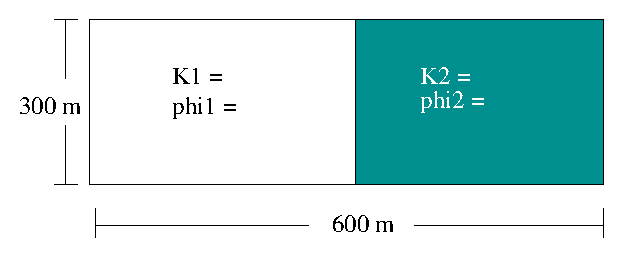
\includegraphics[width=0.5\linewidth,keepaspectratio]{EPS/exercise1_c.eps}
\caption{Exercise 1d: Set-up of a model domain a heterogeneity. $\Delta \text{x} = 20$ m $\Delta \text{y} = 20$ m.}\label{tutorial-coupled:exercise1_d}
\end{figure}

\end{enumerate}

\subsubsection{Exercise 2}
For this exercise you should create a new proplem file analogous to
the file \texttt{tutorialproblem\_coupled.hh} and a new soil property
file just like \texttt{tutorialsoil\_coupled.hh}. These files need to
be included in the file \texttt{tutorial\_coupled.cc}. 

The new soil file should contain the definition of a new soil class
e.g. \texttt{SoilEx2}. Make sure that you also adjust the guardian
macros in the header files (e.g. change \texttt{TUTORIAL\_SOIL} to
\texttt{TUTORIAL\_SOILEX2}).  The new problem file should define and
use a new type tag for the problem as well as a new problem class
e.g. \texttt{ProblemEx2}. Make sure you assign your newly defined soil
class to the \texttt{Soil} property for the new type tag. Just like
for your new soil, you also need to adjust the guardian macros in the
problem file.

After this, change the \texttt{create()} method of the \texttt{Grid}
property and your soil class, so that it matches the domain described
by figure \ref{tutorial-coupled:ex2_Domain}. Adapt the problem class
so the boundary conditions are consistent with figure
\ref{tutorial-coupled:ex2_BC}. Initially the domain is fully saturated
with water and the pressure is $p_w = 5 \times 10^5 \text{Pa}$ . Oil
infiltrates from the left side. Create a grid with $20$ cells in
$x$-direction and $10$ cells in $y$-direction. The simulation time
should be set to $4\times 10^7 \text{s}$ with an inital time step of
$100 \text{s}$.

Now include your new problem file in the main file and replace the
\texttt{TutorialProblemCoupled} type tag by the one you've created and
compile the program.


\begin{figure}[h]
\psfrag{K1}{K $= 10^{-7}\text{ m}^2$}
\psfrag{phi1}{$\phi = 0.2$}
\psfrag{Lin}{Linear Law}
\psfrag{K2}{K $= 10^{-9}\text{ m}^2$}
\psfrag{phi2}{$\phi = 0.15$}
\psfrag{BC1}{Brooks Corey Law} 
\psfrag{BC2}{$\lambda = 1.8$, $p_b = 0.0$}
\psfrag{H1y}{50 m}
\psfrag{H2y}{15 m}
\psfrag{H3y}{20 m}
\psfrag{L1x}{100 m}
\psfrag{L2x}{50 m}
\psfrag{L3x}{25 m}
\centering
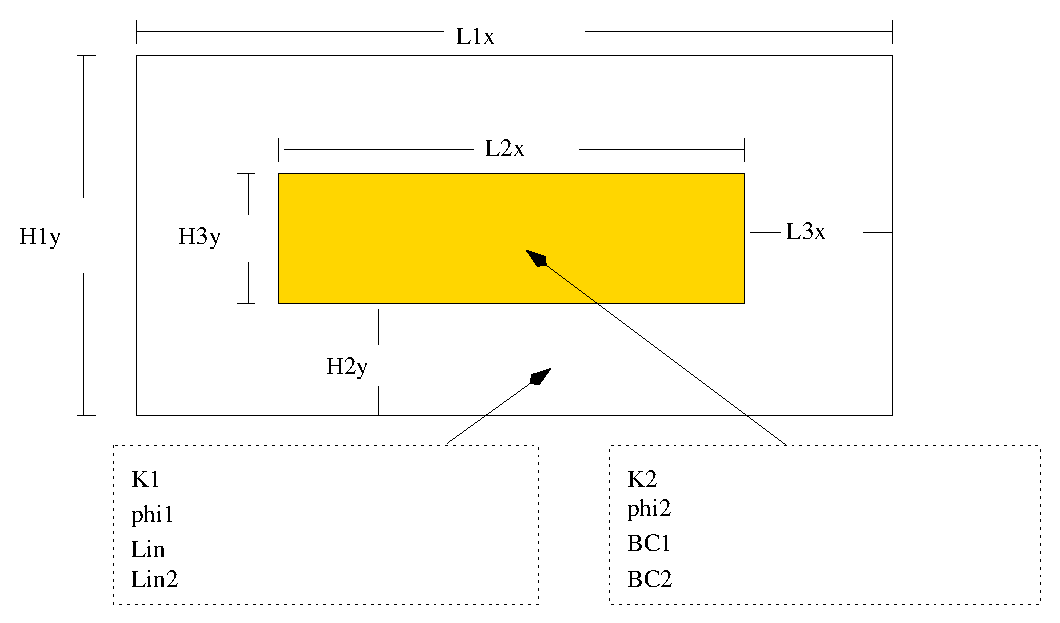
\includegraphics[width=0.8\linewidth,keepaspectratio]{EPS/Ex2_Domain.eps}
\caption{Set-up of the model domain and the soil parameters}\label{tutorial-coupled:ex2_Domain}
\end{figure}

\begin{figure}[h]
\psfrag{pw}{$p_w = 5 \times 10^5$ \text{Pa}}
\psfrag{S}{$S_n = 1.0$}
\psfrag{qw}{$q_w = 2 \times 10^{-4}$ [kg/$\text{m}^2$s]}
\psfrag{qo}{$q_n = 0.0$ [kg/$\text{m}^2$s]}
\psfrag{no flow}{no flow}
\centering
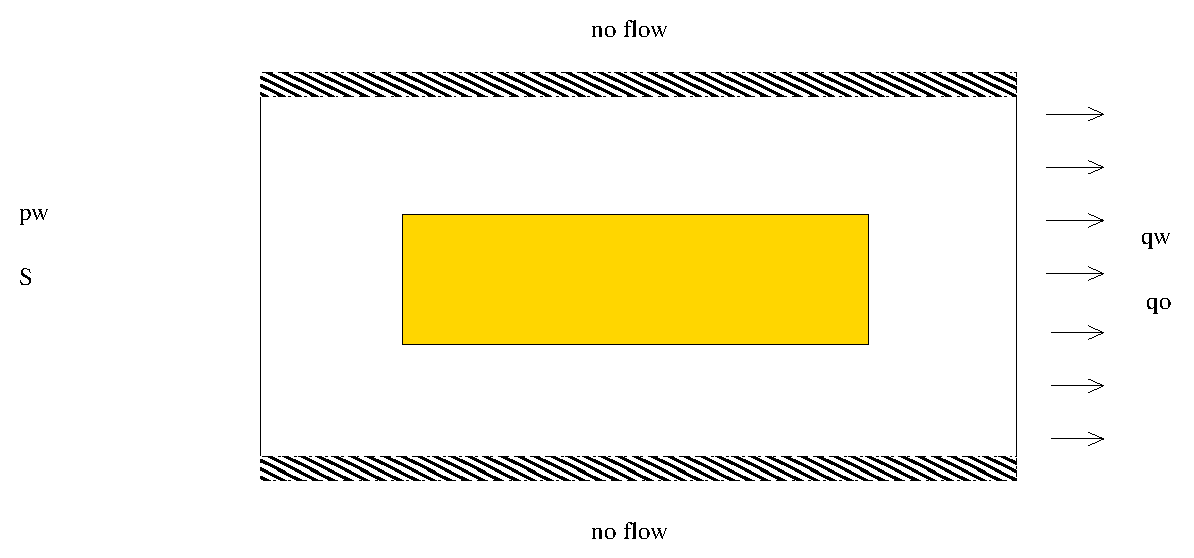
\includegraphics[width=0.8\linewidth,keepaspectratio]{EPS/Ex2_Boundary.eps}
\caption{Boundary Conditions}\label{tutorial-coupled:ex2_BC}
\end{figure}

\subsubsection{Exercise 3}

Create a new file for benzene called \texttt{benzene.hh} and implement
a new fluid class. This new fluid class should be derived from the
base class \texttt{Fluid} located in
\texttt{/dumux/material/property\_baseclasses.hh}.  (You may get a
hint by looking at existing fluid classes in the directory
\texttt{/dumux/material/fluids}.)

Use benzene as a new fluid and run the model of Exercise 2 with water
and benzene. Benzene has the following properties:
\begin{description}
  \item[density:] $889.51 \, \text{kg} / \text{m}^3$
  \item[viscosity:] $0.00112 \, \text{Pa} \; \text{s}$
\end{description}

